\documentclass[aspectratio=169]{beamer}
\usetheme{metropolis}
\metroset{subsectionpage=progressbar}

\usefonttheme{professionalfonts} % 使用系统/自定字体


% === 字体设置 ===
\usepackage[UTF8,scheme=plain,fontset=none]{ctex}
\setCJKmainfont{Source Han Serif CN}[BoldFont={Source Han Serif CN Bold}]
\setCJKsansfont{Source Han Sans CN}[BoldFont={Source Han Sans CN Bold}]
% \setCJKmonofont{Sarasa Mono CN}

% beamer 已加载 hyperref;加 unicode 以支持中文书签
\hypersetup{unicode}

% define paragraph
\providecommand{\paragraph}[1]{\smallskip\textbf{#1}\par}

% 常用包
\usepackage{longtable,booktabs}
\usepackage{amsmath,amssymb}
\usepackage{graphicx}
\usepackage{tikz}
\usetikzlibrary{positioning,arrows.meta}
% \graphicspath{{.}{./figs/}{./images/}{./images_in_paper/}}
\usepackage{caption}
\usepackage{subcaption}
\usepackage{float}
\usepackage{svg}
\usepackage{booktabs}
\usepackage{array}
\usepackage{threeparttable}

% 算法环境(与 beamer 兼容)
\usepackage{algorithm}
\usepackage[noend]{algpseudocode}  % 提供 algorithmic 环境、\State 等
% 可选:微调 algorithmic 缩进
\algrenewcommand\algorithmicindent{0.8em}

% 数学粗体与梯度符号
\usepackage{bm} % \boldsymbol
\newcommand{\bx}{\mathbf{x}}
\newcommand{\bz}{\mathbf{z}}
\newcommand{\bI}{\mathbf{I}}
\newcommand{\bzero}{\mathbf{0}}
\newcommand{\bepsilon}{\boldsymbol{\epsilon}}
\newcommand{\grad}{\nabla}
% 超链接(beamer 已加载 hyperref,这里只补选项)
% \hypersetup{unicode=true}

% 编号风格
\setbeamertemplate{caption}[numbered]
\setbeamertemplate{caption label separator}{.}

\title{基于JiT的diffusion超分辨模型}
\author{李孟霖}
\date{\today}

%---Document Begins---
\begin{document}
\begin{frame}[plain]
  \titlepage
\end{frame}
\section{Introduction}
\subsection{研究背景}

\begin{frame}{主流超分辨模型范式}
\paragraph{回归型方法(Pixel-wise Regression)}
\begin{itemize}
  \item \textbf{EDSR(CNN)}:以 MSE / L1 为目标,PSNR/SSIM 表现稳定
  \item \textbf{SwinIR(Transformer)}:更强建模能力,当前 SR 指标基线
\end{itemize}

\paragraph{生成型方法(Generative Models)}
\begin{itemize}
  \item \textbf{GAN-based SR}(如 SRGAN):提升感知质量,但训练不稳定、指标与视觉存在权衡
  \item \textbf{Diffusion-based SR}(如 SR3、StableSR):逐步去噪,\textbf{高频细节表达能力强}
\end{itemize}

\paragraph{动机}
Diffusion 模型在生成任务中往往具有较强的高频细节建模能力,
本任务中尝试将 \textbf{Diffusion + Transformer backbone} 引入超分辨任务
\end{frame}

\begin{frame}{Diffusion 去噪网络的 Backbone 选择}
\paragraph{常见去噪结构}
\begin{itemize}
  \item \textbf{UNet}:
  多尺度卷积结构,局部归纳偏置强,在超分辨等低层视觉任务中被广泛采用
  \item \textbf{DiT / JiT(Transformer-based)}:
  使用 ViT 结构作为去噪网络,通过 self-attention 建模全局依赖
\end{itemize}

\paragraph{Transformer 的潜在优势}
\begin{itemize}
  \item \textbf{全局建模能力强}:self-attention 可直接建模远距离像素/patch 关系
  \item \textbf{结构灵活}:天然适合 token-level 条件注入(时间、类别或图像条件)
  \item \textbf{统一建模范式}:避免多尺度卷积结构的复杂设计
\end{itemize}

基于以上考虑,本研究采用 \textbf{Transformer 作为 Diffusion 的去噪模块},
并进一步研究其在 \textbf{图像条件超分辨任务} 中的表现与局限。
\end{frame}

\begin{frame}{Diffusion 模型的去噪预测方式}
\paragraph{三种参数化方式}
\begin{itemize}
  \item \textbf{$\epsilon$-prediction}:
  直接预测噪声 $\epsilon$,是早期 Diffusion 模型的常见形式
  \item \textbf{$x$-prediction}:
  预测原始干净图像 $x_0$,更直观,常用于高分辨率生成
  \item \textbf{$v$-prediction}:
  预测速度变量 $v$,在不同噪声强度下具有更稳定的梯度尺度
\end{itemize}
\paragraph{本任务中的实现方式}
\begin{itemize}
  \item 网络前向输出采用 \textbf{$x$-prediction}
  \item 训练时通过固定变换,将 $x$-prediction 转换为 \textbf{$v$-prediction loss}
  \item 该做法与 JiT / EDM 等工作保持一致
\end{itemize}
\end{frame}

\begin{frame}{v-prediction 的定义}
Diffusion 前向过程定义为:
\[
x_t = \alpha_t x_0 + \sigma_t \epsilon,
\quad \epsilon \sim \mathcal{N}(0, I)
\]

\textbf{v-prediction} 定义为:
\[
v_t = \alpha_t \epsilon - \sigma_t x_0
\]

在训练中,模型预测 $\hat{x}_0$,
并通过固定变换得到 $\hat{v}_t$,
使用 $v$-prediction loss 进行优化。
\end{frame}

\subsection{相关工作}
\begin{frame}{JiT}
  何恺明团队CFG条件生成模型(JiT),Back to Basics: Let Denoising Generative Models Denoise

  低维流形假设:JiT研究认为,真实分布处在整个图像空间中的低维流形中。

  以vit为核心去噪模块替代UNet,模型做x-prediction,x-prediction的预测值变换为v-prediction构造损失函数
\end{frame}


% \begin{frame}{JiT:x-prediction 与 v-prediction}
% \paragraph{JiT 的基本思想}
% JiT(Back to Basics: Let Denoising Generative Models Denoise)认为,
%
% 真实数据分布位于高维图像空间中的\textbf{低维流形},
%
% 使用 Transformer(ViT)作为 Diffusion 的去噪网络。
%
% \end{frame}

\begin{frame}{JiT:x-prediction 与 v-prediction}
\vspace{-0.5em}
前向加噪过程
\[
x_t = t \, x_0 + (1 - t)\, \epsilon,
\quad \epsilon \sim \mathcal{N}(0, I)
\]

\vspace{-0.8em}
模型预测 $\hat{x}_0$,并通过固定变换构造 $v$:
\[
\hat{v}_t = \frac{\hat{x}_0 - x_t}{1 - t},
\qquad
v_t = \frac{x_0 - x_t}{1 - t}
\]

\vspace{-0.8em}
训练目标:
\[
\mathcal{L}
=
\mathbb{E}\!\left[
\left\|
\hat{v}_t - v_t
\right\|_2^2
\right]
\]
\end{frame}

\section{Methods}
\begin{frame}{模型概览}
  主体与JiT相同,去噪模块做x-prediction,换算为v-prediction构造loss

  去噪模块为多个vit模块的串联,串联长度由超参数控制
  
  删去CFGtoken拼接,尝试按下述两种方式将低清图信息引入 
\end{frame}
\begin{frame}{低清图插入方式}
  \begin{itemize}
    \item 将低清图和带噪声图像按通道拼接
    \item 将低清图编码为token,和带噪声图像拼接成一个序列
  \end{itemize}
\end{frame}

\section{实验}
\subsection{性能指标}
\begin{frame}{通道拼接(Concat)方案:性能指标}
\vspace{-0.5em}

\begin{center}
\textbf{PSNR: 6.98 \quad\quad SSIM: 0.146}
\end{center}

\vspace{-0.5em}
\begin{figure}
  \centering
  \includegraphics[width=0.9\linewidth]{./preprocess/figures/L16_concat_curves.pdf}
  \caption{L16 通道拼接方案在验证集上的性能曲线}
\end{figure}
\end{frame}

\begin{frame}
\begin{figure}
  \centering
  \includegraphics[width=0.9\linewidth]{./preprocess/figures/L16_concat_img.png}
  \caption{L16 通道拼接方案效果图}
\end{figure}
\end{frame}

\begin{frame}{Token 拼接方案:性能指标}
\vspace{-0.5em}

\begin{center}
\textbf{PSNR: 20.47 \quad\quad SSIM: 0.617 \quad\quad 参数量: 131M}
\end{center}

\vspace{-0.5em}
\begin{figure}
  \centering
  \includegraphics[width=0.9\linewidth]{./preprocess/figures/B16_token_curves.pdf}
  \caption{B16 Token 拼接方案在验证集上的性能曲线}
\end{figure}
\end{frame}

\begin{frame}
\begin{figure}
  \centering
  \includegraphics[width=0.9\linewidth]{./preprocess/figures/L16_token_img.png}
  \caption{B16 token拼接方案效果图}
\end{figure}
\end{frame}
\begin{frame}{Token 拼接方案:性能指标}
\vspace{-0.5em}

\begin{center}
\textbf{PSNR: 21.10 \quad\quad SSIM: 0.634 \quad\quad 参数量: 462M}
\end{center}

\vspace{-0.5em}
\begin{figure}
  \centering
  \includegraphics[width=0.9\linewidth]{./preprocess/figures/L16_token_curves.pdf}
  \caption{L16 Token 拼接方案在验证集上的性能曲线}
\end{figure}
\end{frame}

\begin{frame}
\begin{figure}
  \centering
  \includegraphics[width=0.9\linewidth]{./preprocess/figures/L16_token_img.png}
  \caption{L16 token拼接方案效果图}
\end{figure}
\end{frame}


\section{结果分析}

\begin{frame}{性能对比}
  \begin{table}[]
    \centering
    \begin{tabular}{|c|c|c|}
    \hline
    \textbf{算法}          & \textbf{psnr}       & \textbf{ssim}     \\ \hline
    bicubic       & 19.67      & 0.579     \\ \hline
    EDSR          & 22.92      & 0.702     \\ \hline
    SRGAN         & 21.87      & 0.692     \\ \hline 
    SwinIR        & 23.77      & 0.733     \\ \hline 
    本模型        & 20.47      & 0.617      \\ \hline
    \end{tabular}
    \caption{性能对比}
  \end{table}
\end{frame}

\begin{frame}{整体性能总结}
\begin{itemize}
  \item 在 ImageNet $\times4$ 超分辨任务上,
  本方法在 \textbf{PSNR} 与 \textbf{SSIM} 指标上
  \textbf{明显优于 bicubic 插值}。
  
  \item 与经典回归型超分模型(如 \textbf{EDSR}、\textbf{SwinIR})相比,
  当前模型在 \textbf{PSNR / SSIM 指标上仍存在差距}。
  
  \item 该结果表明:
  基于 Diffusion 的 JiT-SR 方法在像素级重建指标上
  \textbf{尚未达到当前主流 SR 方法的性能水平}。
\end{itemize}
\end{frame}


\begin{frame}{反思:连续型生成模型与重建任务的适配性}
\begin{itemize}
  \item 本工作采用的 Diffusion / JiT 属于 \textbf{连续型生成模型},
  其核心目标是学习条件分布 $p(x_{\text{HR}} \mid x_{\text{LR}})$,
  而非最小化像素级误差。

  \item 对于超分辨这类 \textbf{重建型任务},
  PSNR 与 SSIM 本质上衡量的是
  \textbf{条件均值解的像素一致性},
  与生成模型的优化目标并不完全一致。

  \item 在 ImageNet 等高复杂度数据集上,
  同一低清图像可能对应多种合理的高分辨结果,
  连续型模型更倾向于生成 \textbf{感知上合理但非像素最优} 的样本。

  \item 因此,Diffusion 模型在感知质量与细节多样性上具有优势,
  但在 PSNR / SSIM 等像素级重建指标上
  \textbf{不一定占优},这一现象具有一定的范式必然性。
\end{itemize}
\end{frame}

\begin{frame}{反思:低清图条件信息引入方式}
    简单的token拼接的条件信息引入形式,会导致条件信息token和带噪声图patch的token,在self attention的Q K V中没有区别,
    它们完全对等地“互相参考”
  \begin{figure}
    \centering
    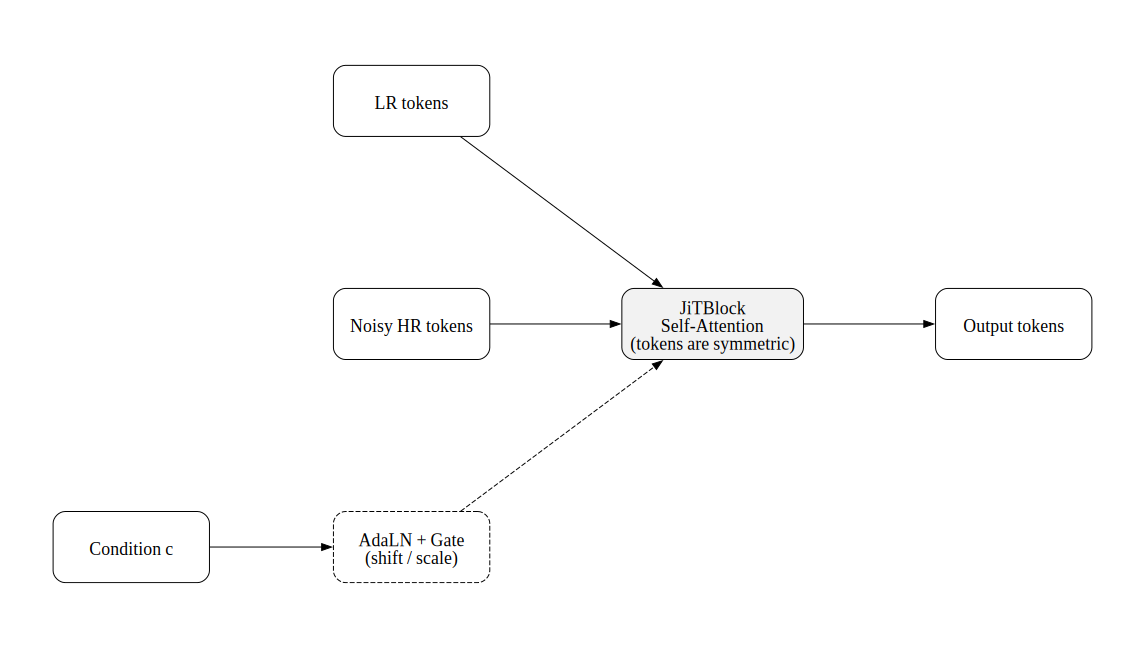
\includegraphics[width=0.65\linewidth]{./preprocess/jitblock_selfAttn.pdf}
    \caption{JitBlock self attention的结构}
  \end{figure}
\end{frame}
\begin{frame}[standout]
  谢谢大家!
\end{frame}
\end{document}
